\chapter{Results}\label{chapter:results}

To search for and quantify the significance of the production of signals $\left(V, H, \Zprime\right)$, and to set limits in the absence of observation, a Bayesian method is used to calculate a posterior likelihood as a function of number of signal events for the signal hypotheses under consideration~\cite{EXOT-2010-07}.
In this method, a final conditional probability of the parameters of interest given the observed data (the ``posterior'') is built by integrating over the nuisance parameters (``marginalization'') with a Markov Chain Monte Carlo (\Gls{MCMC}) procedure.
The posterior distribution is used to gauge the fitted signal statistical significance and to set $95\%$ credibility level (CL)%
\footnote{As discussed in \Cref{section:intervals_and_limits}, \emph{credibility levels} for Bayesian credible intervals are different from \emph{confidence levels} for frequentist confidence intervals.}
upper limits on the cross-section times acceptance times efficiency.

\section{Measurement of Standard Model Signals}

To measure the Standard Model signals a model comprised of the Standard Model $\Vjets$, $\Hbb$, and $\ttbar$ signal templates along with the QCD multijet model is fit to the data.
The normalization of the $\ttbar$ component of the model is constrained with the scale factor obtained in the dedicated $\ttbar$ Control Region.
This fit simultaneously extracts the signal strengths of the $\Vjets$ and $\Hbb$ process, $\mu_{V}$ and $\mu_{H}$ respectively, which are unconstrained.
The comparison of the model post marginalization of the nuisance parameters to the data is seen in \Cref{fig:post_fit}.

\begin{figure}[htbp]
 \centering
 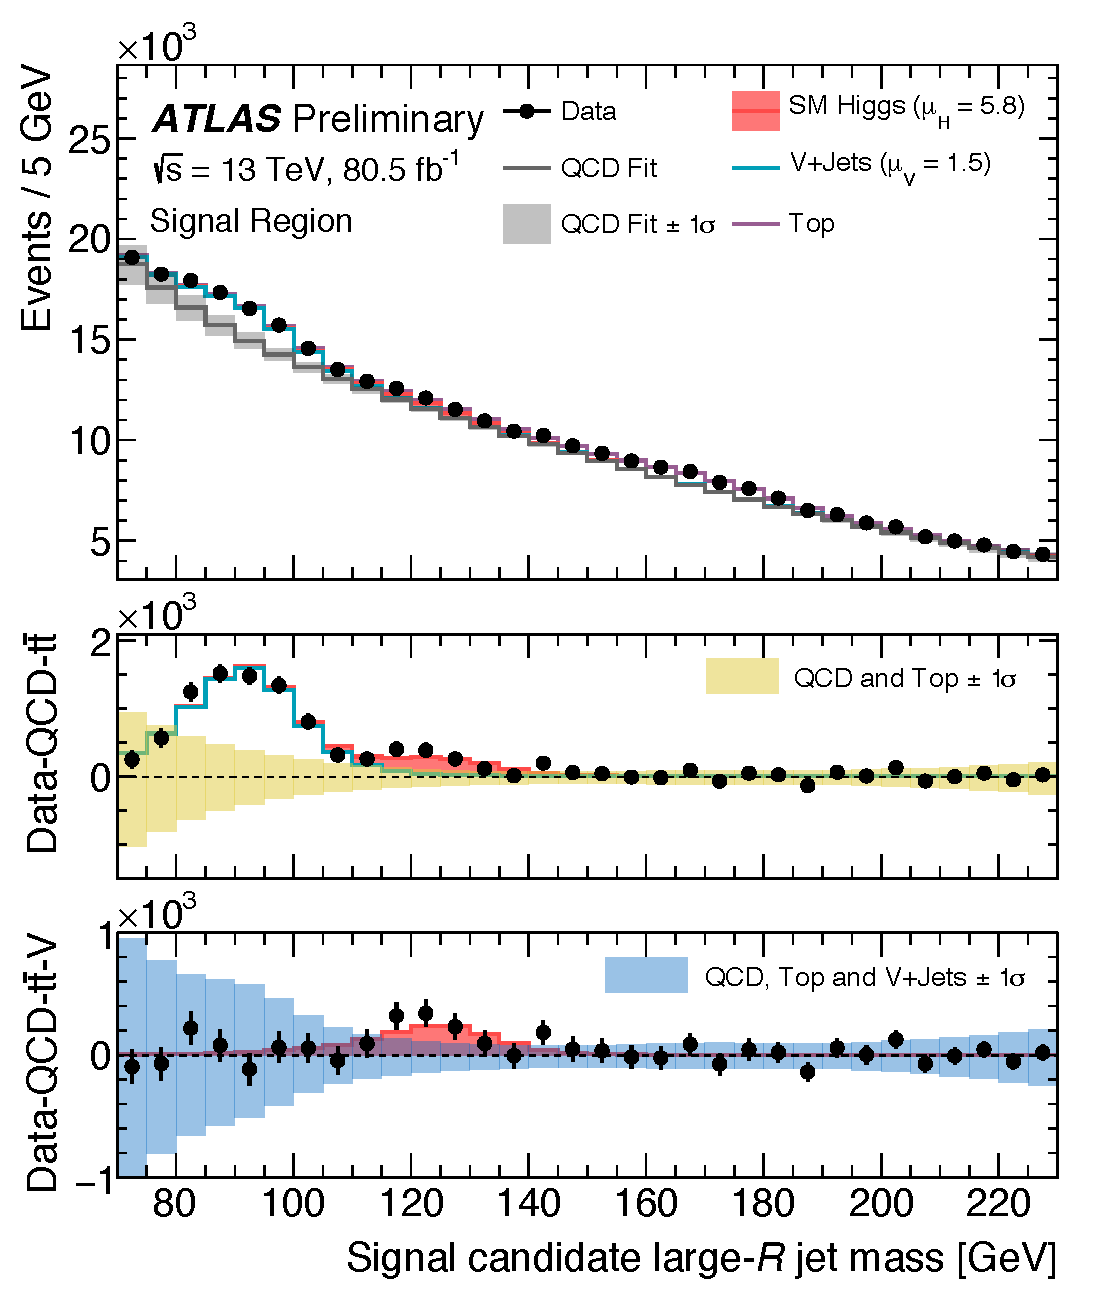
\includegraphics[width=\linewidth]{results/SRPostFit_mass}
 \caption[Plot of post-fit model with observed data and with model components subtracted.]{%
  The top panel shows the post-fit plot of the SM Higgs boson, $\Vjets$, $\ttbar$ and QCD model with the observed data.
  The middle panel shows the post-fit model and the data with the QCD and $\ttbar$ components of the model subtracted, highlighting the large resonance from $\Vjets$.
  The bottom panel shows the post-fit model and the data with the QCD, $\Vjets$, and $\ttbar$ components of the model subtracted, highlighting a small excess of events near $125~\GeV$~\cite{ATLAS-CONF-2018-052}.
 }
 \label{fig:post_fit}
\end{figure}

\subsection{Observation of boosted $V\to b\bar{b}$}

The observed signal strength for the $\Vjets$ process is
\[
 \mu_{V} = 1.5 \pm 0.22~\mathrm{(stat.)}^{+0.29}_{-0.25}~\mathrm{(syst.)} \pm 0.18~\mathrm{(th.)}\,,
\]
corresponding to an observed significance of $5\,\sigma$ with an expected significance of $4.8\,\sigma$.
This constitutes the first direct observation of boosted vector bosons decaying to bottom quark pairs in ATLAS for a center-of-mass energy of $\sqrt{s}=13~\TeV$ following the lower momentum Run-I measurement of high transverse momentum $\Zbb$~\cite{STDM-2013-04}.

\subsection{Measurement of boosted $H\to b\bar{b}$}

For the $\Hbb$ process, the observed signal strength is
\[
 \mu_{H} = 5.8 \pm 3.1~\mathrm{(stat.)} \pm 1.9~\mathrm{(syst.)} \pm 1.7~\mathrm{(th.)}\,,
\]
which given the uncertainties is consistent with the background-only hypothesis at $1.6\,\sigma$ with an expected sensitivity of $0.28\,\sigma$.
This constitutes a measurement of boosted Higgs decaying to bottom quark pairs, though not a direct observation.

The combined posterior distributions of $\mu_{V}$ and $\mu_{H}$ is seen in \Cref{fig:signal_strength_contour}, showing the agreement between the best-fit values of the model and the Standard Model prediction of $\mu_{V} = \mu_{H} = 1$.
Given their respective uncertainties, the $\mu_{V}$ best-fit value is compatible with the SM prediction at $1.32\,\sigma$, and the $\mu_{H}$ best-fit value is compatible at $1.2\,\sigma$.

\begin{figure}[htbp]
 \centering
 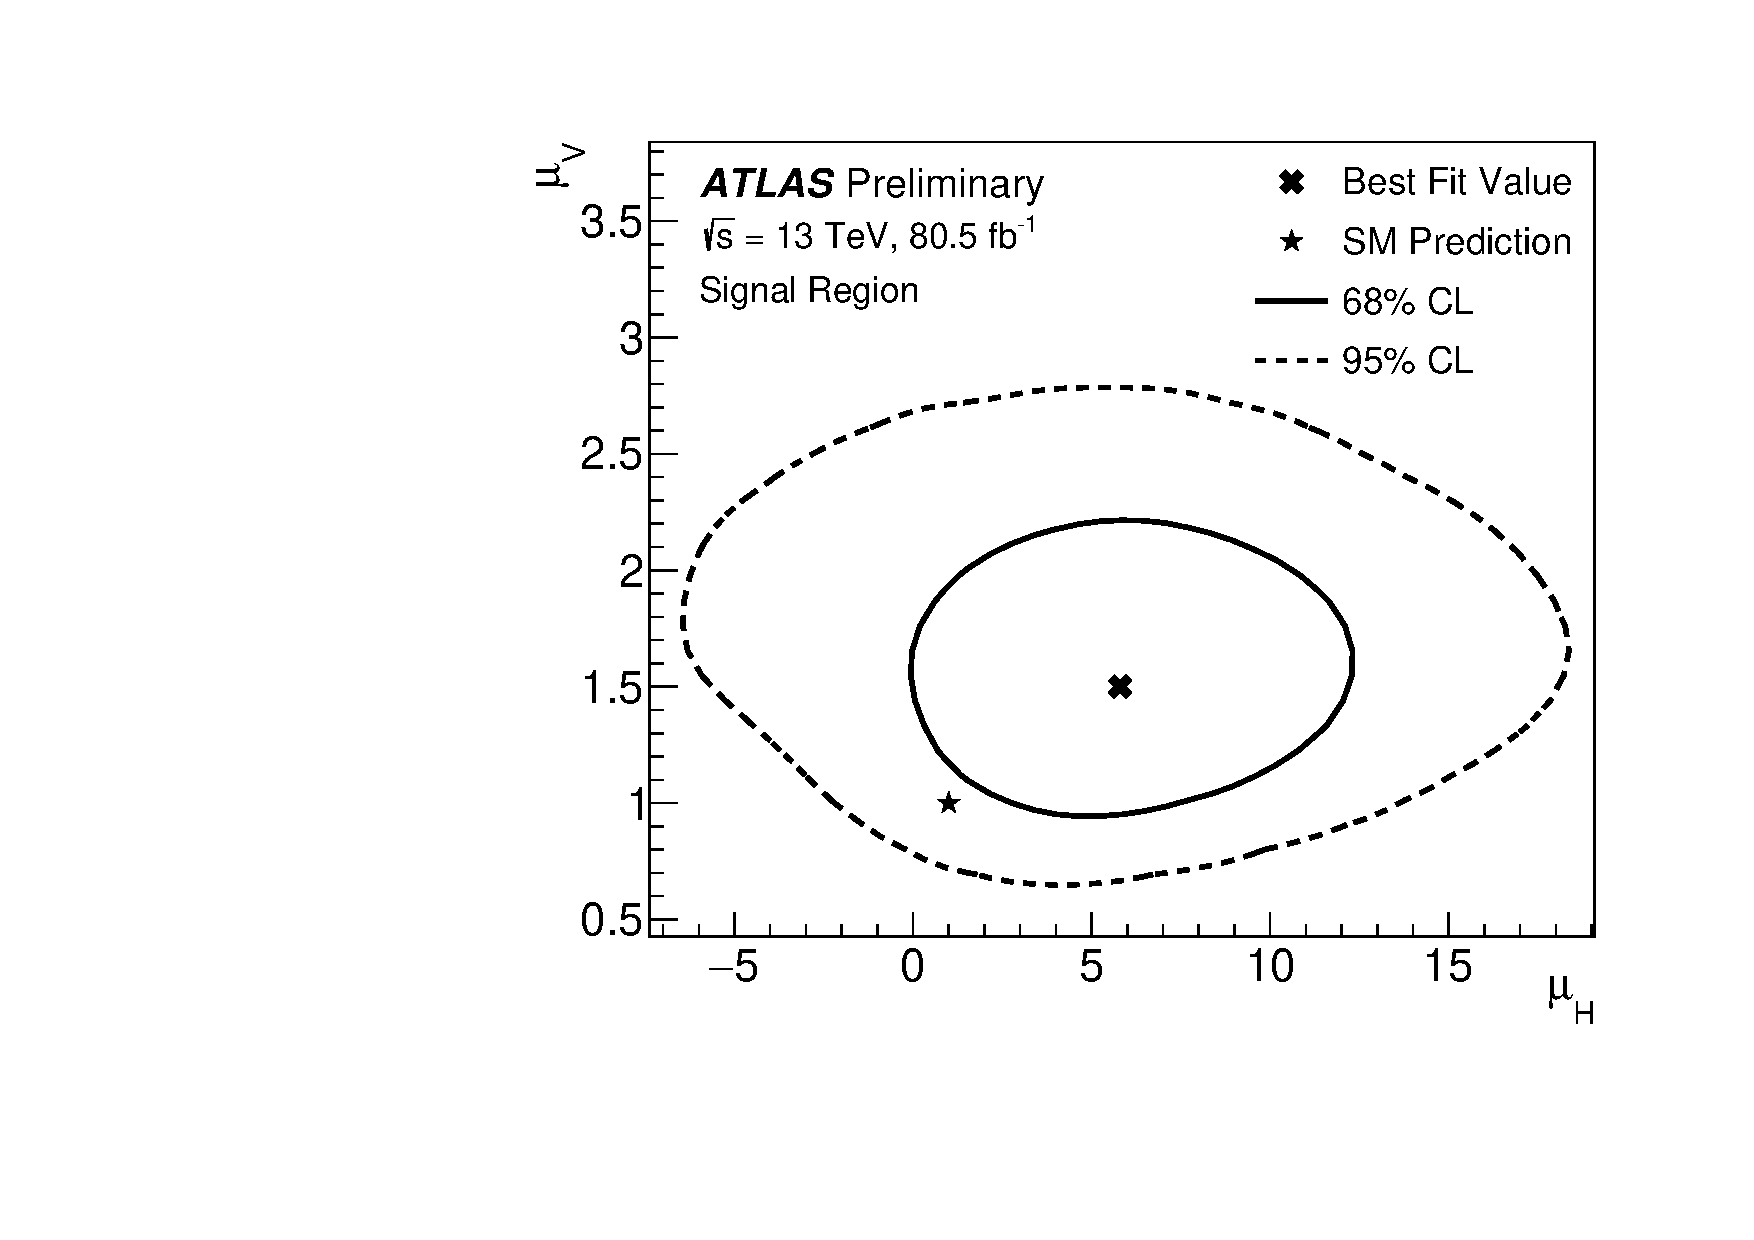
\includegraphics[width=\linewidth]{results/contourFinal}
 \caption[Compatibility of best-fit values for $\mu_{H}$ and $\mu_{V}$ with Standard Model predicted values.]{%
  Combined posterior distributions of $\mu_{H}$ and $\mu_{V}$ from the signal region fit.
  It is seen that the best-fit values for the signal processes lie within the $2\,\sigma$ interval of the Standard Model prediction~\cite{ATLAS-CONF-2018-052}.}
 \label{fig:signal_strength_contour}
\end{figure}
\clearpage

\section{Limits on $\Zprime$ production}

Following the measurement of the Standard Model signals, a search for exotic signals in the \largeR jet mass distribution is performed.
The first step in the search is to apply the \BumpHunter{} search procedure~\cite{Aaltonen:2008vt,Choudalakis:2011qn}.
Given that the effect of the Higgs boson with a SM strength is smaller than the expected uncertainty on the $\Zprime$ limit the SM Higgs template is excluded from the model, and only the $\Vjets$ and $\ttbar$ templates are considered along with the QCD parametric model.
With this model, a fit to the data is performed with the full set of systematic uncertainties resulting in the best-fit values for the model nuisance parameters used in the analysis.
With these post-fit shapes, the \BumpHunter{} goodness-of-fit algorithm scans the mass range looking for significant deviations from the background-only model.
For the given model, the largest deviation from the background is found in the \largeR jet mass interval of $\left[115,130\right]~\GeV$, as seen in \Cref{fig:BumpHunter_scan}.
This deviation has a \BumpHunter{} global \pvalue{} of $0.54$, indicating that background-only model is quite consistent with the data.

The \BumpHunter{} test statistic, described in detail in~\cite{Choudalakis:2011qn}, is calculated for the given model and for pseudo-data sampled from the background only hypothesis (the null hypothesis, $H_{0}$) for various widths of fit windows.
The \BumpHunter{} \pvalue{} is then calculated from the most discrepant test statistic from all the window width choices in a treatment that creates a hypertest --- a union of multiple hypothesis tests --- allowing for accounting of the ``trial factor''~\cite{Gross:2010qma} in the calculation resulting in a global \pvalue{}, making the result quite robust.
For each bin the significance of the deviation between the model and the data is also calculated.
The significance for each bin is defined as the $z$-score for the observed Poisson \pvalue{}~\cite{Choudalakis:2012}, and given the integral form of the relationship between a Normal \pvalue{}, $p$, and the $z$-score, $z$,
\[
 p = \int_{z}^{\infty} \frac{1}{\sqrt{2\pi}}\,e^{-t^2/2}\,dt = 1 - \mathrm{CDF}\left(z\right) = \frac{1}{2}\left(1 - \mathrm{erf}\left(\frac{z}{\sqrt{2}}\right)\right)\,,
\]
shown in \Cref{fig:pvalues_from_zscores}, it is seen the $z$-score can be described numerically%
\footnote{The error function does not have a closed form solution.}
as
\[
 z\textrm{-score} = \sqrt{2}\, \mathrm{erf}^{-1}\left(1-2p\right).
\]

\begin{figure}[htbp]
 \centering
 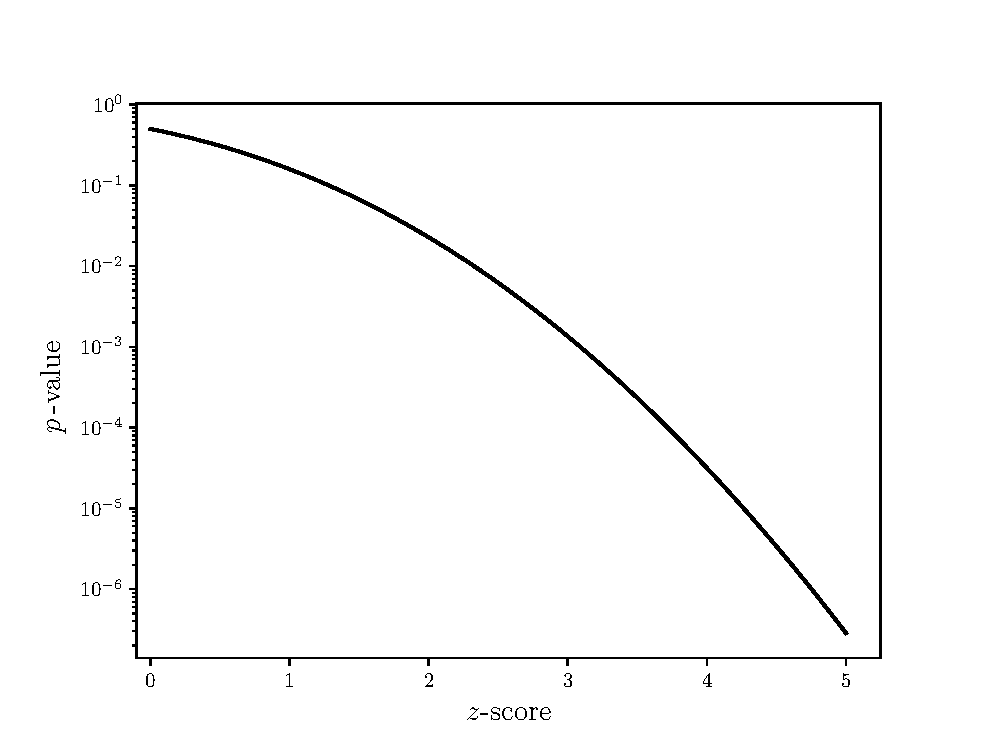
\includegraphics[width=0.575\linewidth]{results/pvalues_from_zscores.eps}
 \caption[Plot of \pvalue{} as a function of $z$-score.]{%
  Plot of $\frac{1}{2}\left(1 - \mathrm{erf}\left(z/\sqrt{2}\,\right)\right)$, which describes the corresponding \pvalue{} for a given $z$-score.}\label{fig:pvalues_from_zscores}
\end{figure}

In the absence of excesses in the data that could correspond to new physics, $95\%$ credibility level upper limits, competitive with other published ATLAS limits~\cite{EXOT-2017-32}, are set on signals from dark matter mediators with democratic decays to quarks for masses between $100~\GeV$ and $200~\GeV$.
These limits are shown in \Cref{fig:Zprime_limits}, in terms of cross section times branching ratio, acceptance and efficiency (\Cref{fig:cross_section_limits}), and in terms of the $g_{q}$ parameter%
\footnote{The limits on $g_{q}$ are determined from the limits on $\sigma \times \epsilon \times A \times BR$ which used signal events simulated with $g_{q} = 0.25$, meaning that as $\sigma\left(\Zprime \to q\bar{q}\right) \propto g_{q}^{2}$ that $g_{q} = 0.25 \sqrt{\sigma/\sigma_{g_{q} = 0.25}}$\,.}
that controls the coupling of the \gls{dark matter mediator} to quarks that determines the cross-section (\Cref{fig:gq_limits}).
From these limits, an exotic dark matter mediator $\Zprime$ with $g_{q}=0.25$ is excluded for $m_{\Zprime} < 200~\GeV$ at the $95\%~\mathrm{CL}$.
As in seen in \Cref{fig:gq_limits}, the smallest coupling to quarks excluded at the $95\%~\mathrm{CL}$ is $g_{q} = 0.124$ for a mass hypothesis of $m_{\Zprime} = 105~\GeV$.
The limits become less restrictive at higher masses as the systematic uncertainty on the $t\bar{t}$ scale factor becomes dominant and greatly affects the total uncertainty, as seen in \Cref{table:systematic_uncertainties}.

\begin{figure}[htbp]
 \centering
 \begin{subfigure}[t]{0.5\textwidth}
  \centering
  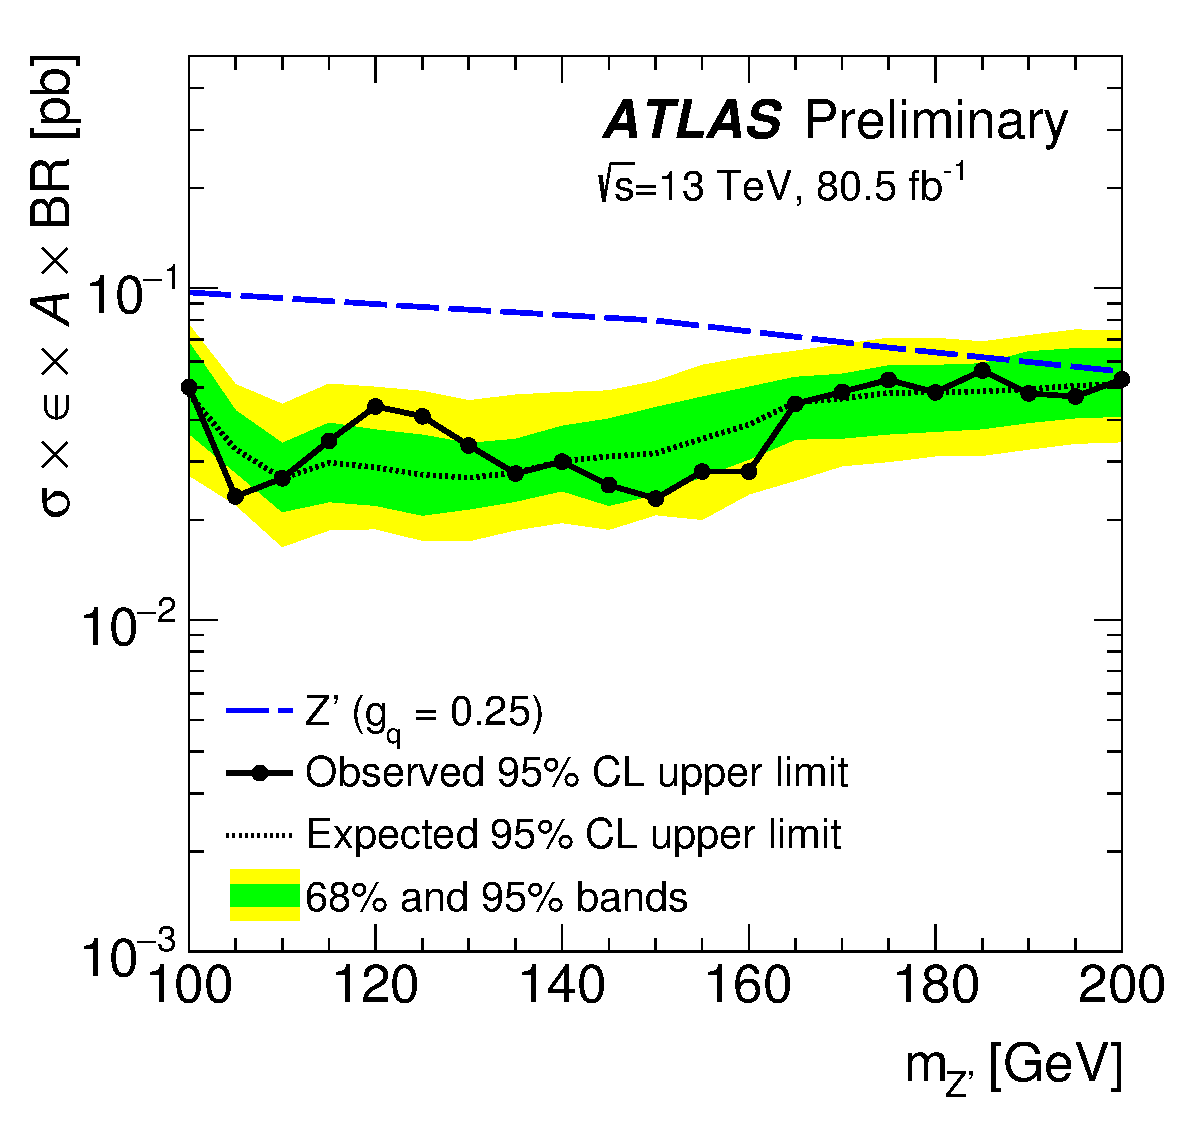
\includegraphics[width=\textwidth]{results/Final_Limits}
  \caption{The limit on the cross-section times acceptance times branching ratio times efficiency.}
  \label{fig:cross_section_limits}
 \end{subfigure}%
 ~
 \begin{subfigure}[t]{0.5\textwidth}
  \centering
  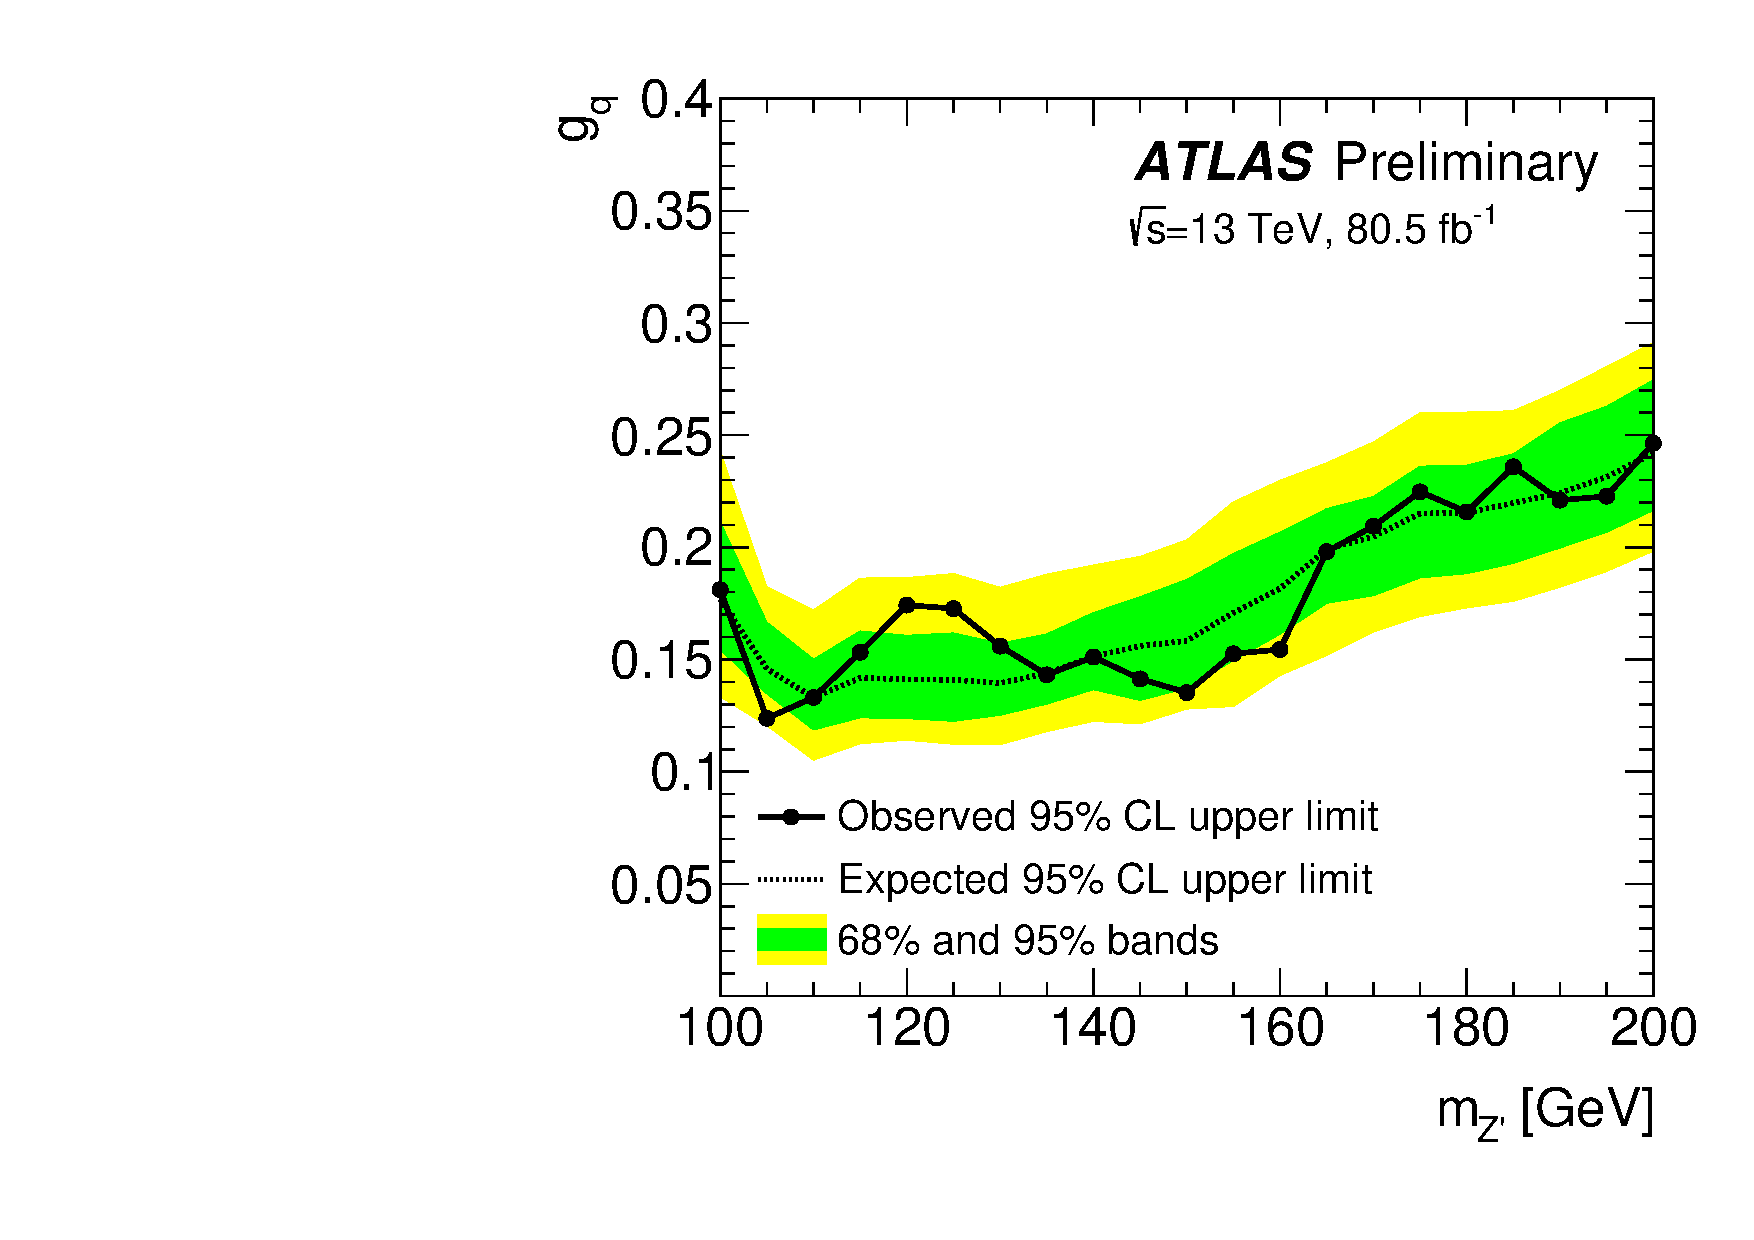
\includegraphics[width=\textwidth]{results/gqlimit}
  \caption{The limit on the $g_{q}$ parameter that controls the decay width of the $\Zprime$ into SM quarks.}
  \label{fig:gq_limits}
 \end{subfigure}
 \caption[The $95\%$ credibility level upper limits obtained from the invariant mass distribution for the $\Zprime$ dark matter mediator model.]{%
  The $95\%$ credibility level upper limits obtained from the invariant mass distribution for the $\Zprime$ dark matter mediator model~\cite{ATLAS-CONF-2018-052}.}
 \label{fig:Zprime_limits}
\end{figure}

\clearpage
\begin{figure}[htbp]
 \centering
 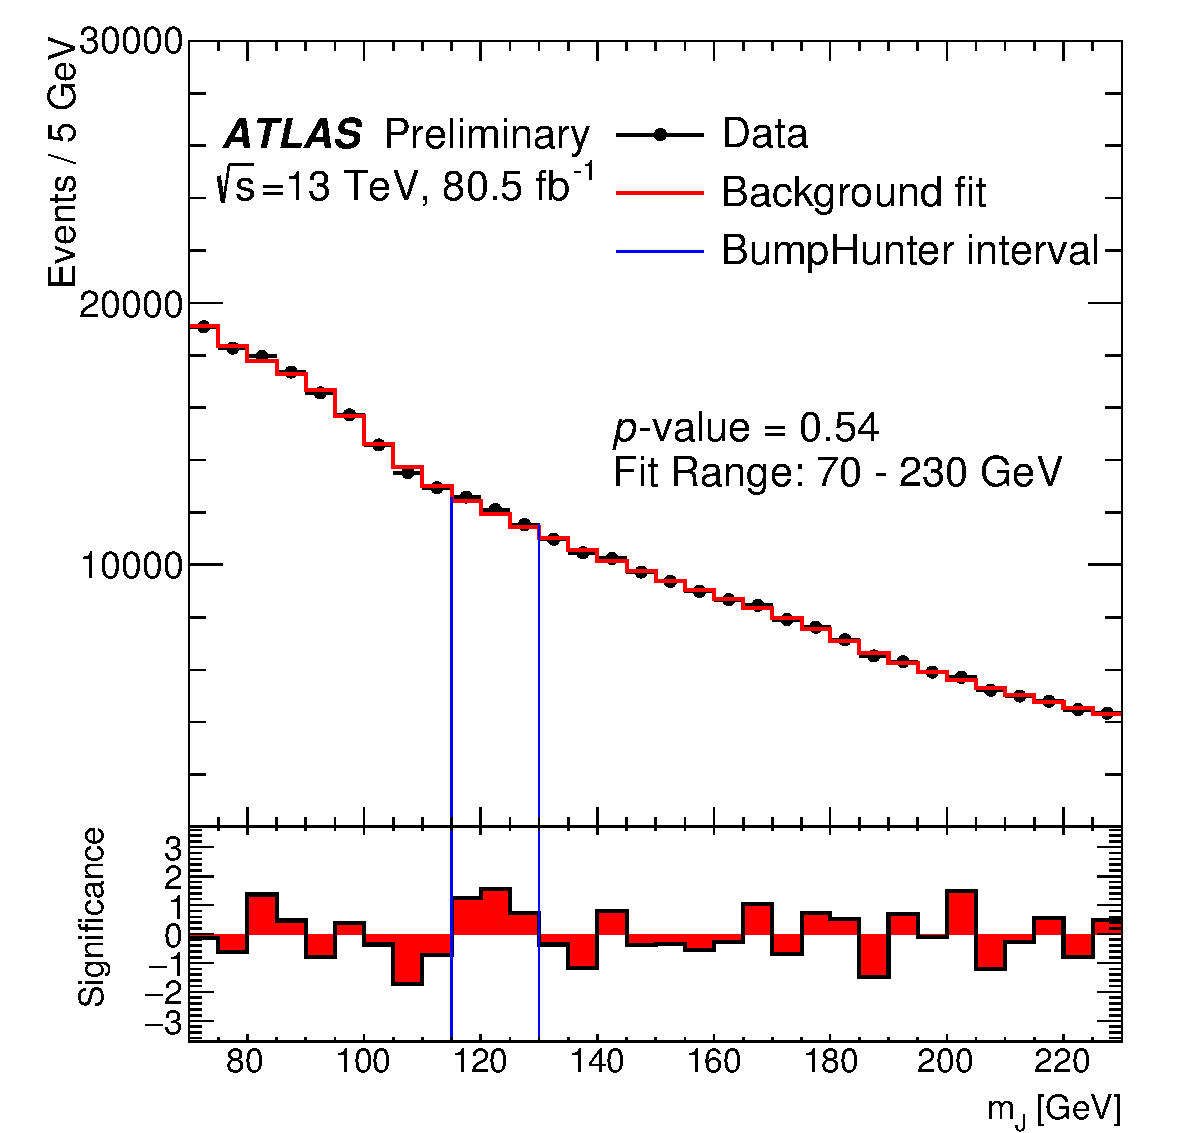
\includegraphics[width=\linewidth]{results/BH_final}
 \caption[\BumpHunter{} fit of post-fit background-only model to data.]{%
  The reconstructed mass distribution $m_{J}$ with the event reconstruction and selection as described in the text.
  The solid red line depicts the background prediction, consisting of the non-resonant dijet, $\Vjets$, and $\ttbar$ processes.
  The vertical blue lines indicate the most discrepant interval identified by the \BumpHunter{} algorithm between $115~\GeV$ and $130~\GeV$.
  Without including systematic uncertainties, the probability that fluctuations of the background model would produce an excess at least as significant as the one observed in the data anywhere in the distribution, the \BumpHunter{} probability, is $0.54$.
  The bottom panel shows the bin-by-bin significances~\cite{Choudalakis:2012} of the differences between the data and the fit, considering only statistical fluctuations~\cite{ATLAS-CONF-2018-052}.
 }
 \label{fig:BumpHunter_scan}
\end{figure}
